\subsubsection{Berechnung Horizontale Ausrichtung}
In der Tabelle \ref{tab:glossarHorizontaleAusrichtung} sind die benötigten
Formelzeichen mit deren Bedeutung aufgelistet, die für die Berechnung der horizontalen
Ausrichtung benötigt werden.
\begin{table}[h!]
    \begin{tabular}{lcl}
        \rule{0pt}{11pt}Zeichen & Einheit & Bezeichnung \\
        \hline\rule{0pt}{11pt}$F_{Losteil}$ & $N$ & Gewichtskraft der Losteile \\
        \rule{0pt}{11pt}$m_{Losteil}$ & $kg$ & Gewicht der Losteile \\
        \rule{0pt}{11pt}$g$ & $\frac{N}{kg}$ & Erdgravitation \\
        \rule{0pt}{11pt}$F_2$ & $N$ & Normalkraft bei den Kugelrollen \\
        \rule{0pt}{11pt}$M_{Drehung}$ & $Nm$ & Drehmoment ausgeübt am Drehpunkt \\
        \rule{0pt}{11pt}$L$ & $m$ & Abstand Drehpunkt zu Kugelrollen \\
        \rule{0pt}{11pt}$F_{R2}$ & $N$ & Reibkraft zwischen Kugelrolle und Spielfeld \\
        \rule{0pt}{11pt}$\mu_H$ & $1$ & Haftreibungskoeffizient zwischen Kugelrolle und Boden \\
        \rule{0pt}{11pt}$M_{Motor}$ & $Nm$ & Drehmoment des einzusetzenden Motors \\
        \rule{0pt}{11pt}$F_Z$ & $N$ & Kraft an den Zahnklanke des Antriebsritzels \\
        \rule{0pt}{11pt}$r$ & $m$ & Radius des Antriebsritzel \\
        \rule{0pt}{11pt}$R$ & $m$ & Radius Zahnsegment \\
    \end{tabular}
    	\centering
    	\caption{Glossar für die Berechnung der horizontalen Ausrichtung}
    	\label{tab:glossarHorizontaleAusrichtung}
\end{table}
\newpage

\begin{figure}[h!]
    \begin{minipage}[hbt]{0.5\textwidth}
    	Für die Stelleinheit wird ein Schrittmotor eingesetzt. Der Antriebsstrang muss 
    	hinsichtlich Drehmoments ausgelegt werden. Die Grösse des Antriebsritzel wurden 
    	so gewählt, dass ein möglichst leichter Schrittmotor verwendet werden kann. 
    	\begin{align}
    	    F_{Losteil} &= m_{Losteil} \cdot g\\
    	    F_2 &= F_{Losteil} \cdot 0.1\\
    	\end{align}
    	\begin{align}
    	    M_{Drehung} &= L \cdot F_{2R}\\
    	    F_{2R} &= \mu_H \cdot F_2\\
    	\end{align}
    	\begin{align}
    	    M_{Motor} &= F_z \cdot r\\
    	    F_z &= \frac{M_{Drehung}}{R}\\
    	    M_{Motor} &=\frac{L \cdot \mu_H \cdot m_{Losteil} \cdot g \cdot 0.1}{R} \cdot r
    	\end{align}
    	
    	\textbf{Berechnungswerte}\\
    	\begin{tabular}{llp{4cm}}
    		\rule{0pt}{11pt} $m_{Losteil}$ & $1.6 kg$ & \\
    		\rule{0pt}{11pt} $g$ & $9.81 \frac{N}{kg}$ & \\
    		\rule{0pt}{11pt} $L$ & $0.437 m$ &  \\
    		\rule{0pt}{11pt} $\mu_H$ & $0.2$ & Haftreibungskoeffizient zwischen Rolle und Boden \\
    		\rule{0pt}{11pt} $r$ & $0.01 m$ & \\
    		\rule{0pt}{11pt} $R$ & $0.28 m$ & \\
    	\end{tabular}\\
    	\\
    	\\
    	\textbf{Resultate}\\
    	\begin{tabular}{ll}
    		\rule{0pt}{11pt} $M_{motor}$ & $0.0049Nm$ \\
    	\end{tabular}
    \end{minipage}
\hfill
    \begin{minipage}[hbt]{0.5\textwidth}
    	\centering
    	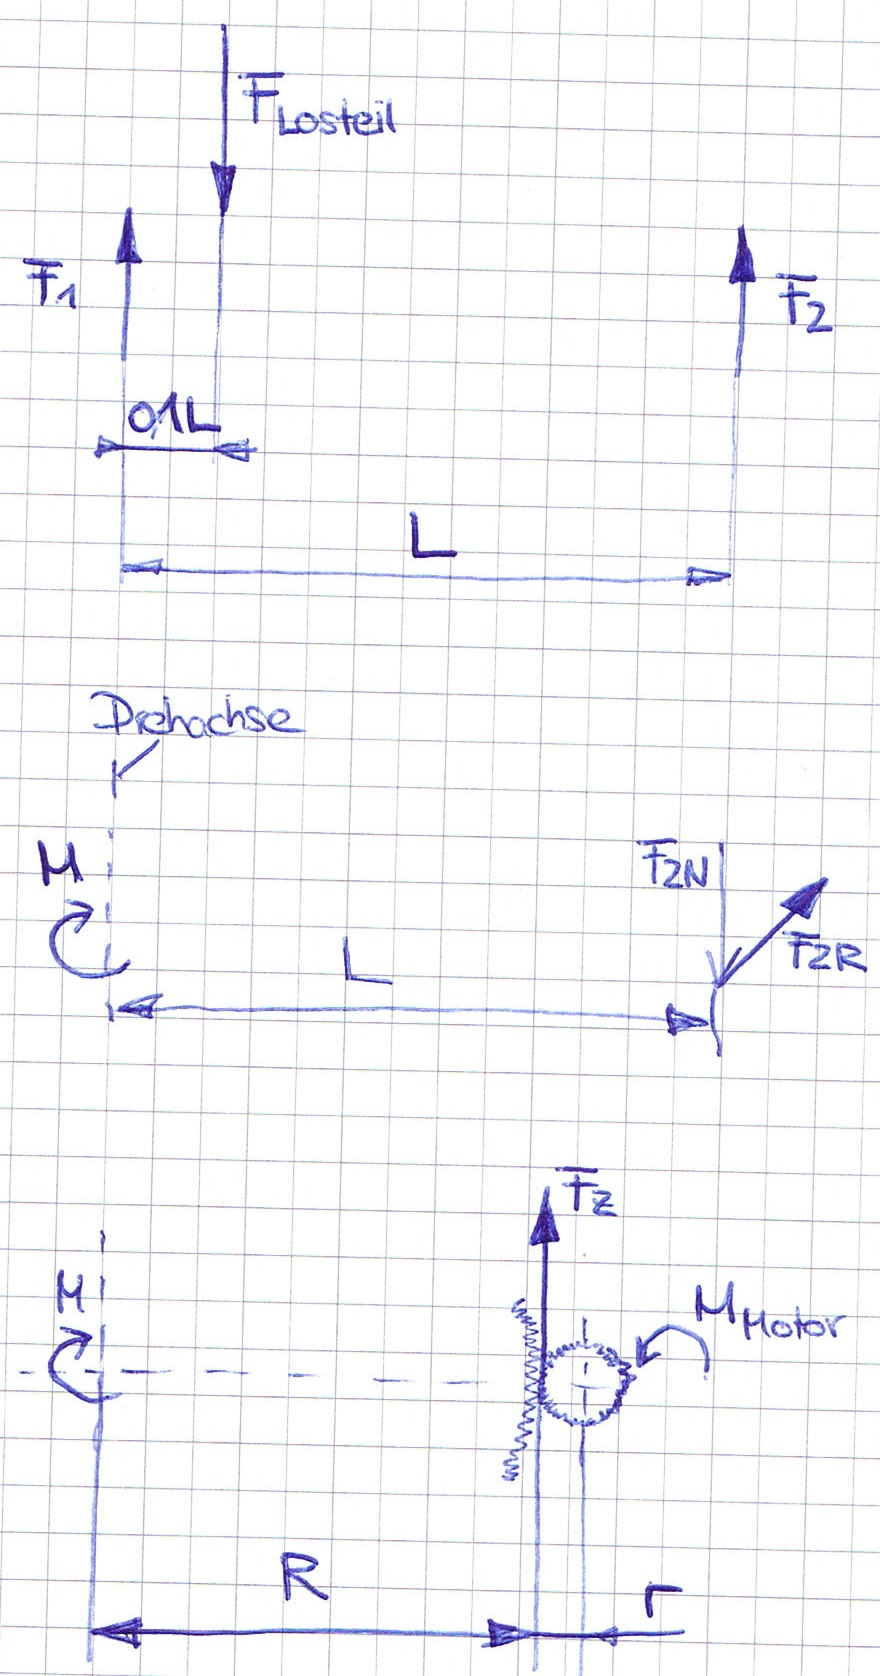
\includegraphics[width=1\textwidth,clip,trim=3cm 0cm 0cm 0cm]
    	{Enddokumentation/Anhang/Bilder/NotizBerechnungDrehmomentStepper.jpg}
    	\caption{Kräftezeichnung der horizontalen Ausrichteinheit}
    	\label{fig:ErklaerungStepper}
    \end{minipage}
\end{figure}
